\section{Argus}
\label{sec:dataset:argus}

Within this section, we present Argus, a partial implementation of our metamodel. We discuss the overall design of Argus and how this fits into the workflow as presented in \cref{sec:dataset:process}. Additionally, we briefly discuss productivity and performance statistics gathered during the data gathering process. Further information related to Argus can be found at \url{http://deakin.edu.au/~ca/argus}.

\subsection{Design}

Argus is designed as a full-screen application to utilise maximum screen space. The application is designed to be keyboard-driven, so shortcuts are displayed wherever possible. Additionally, the current instruction of the workflow is indicated on the top of the image in red to stand out to image taggers. \cref{fig:dataset:argus:overview} shows the main \gls{ui}. Further segment-level features are captured in dialogs or user interaction directly on the image, as shown in \cref{fig:dataset:argus:bib_and_face,fig:dataset:argus:prom_and_col}.

\begin{figure}[h]
  \centering
  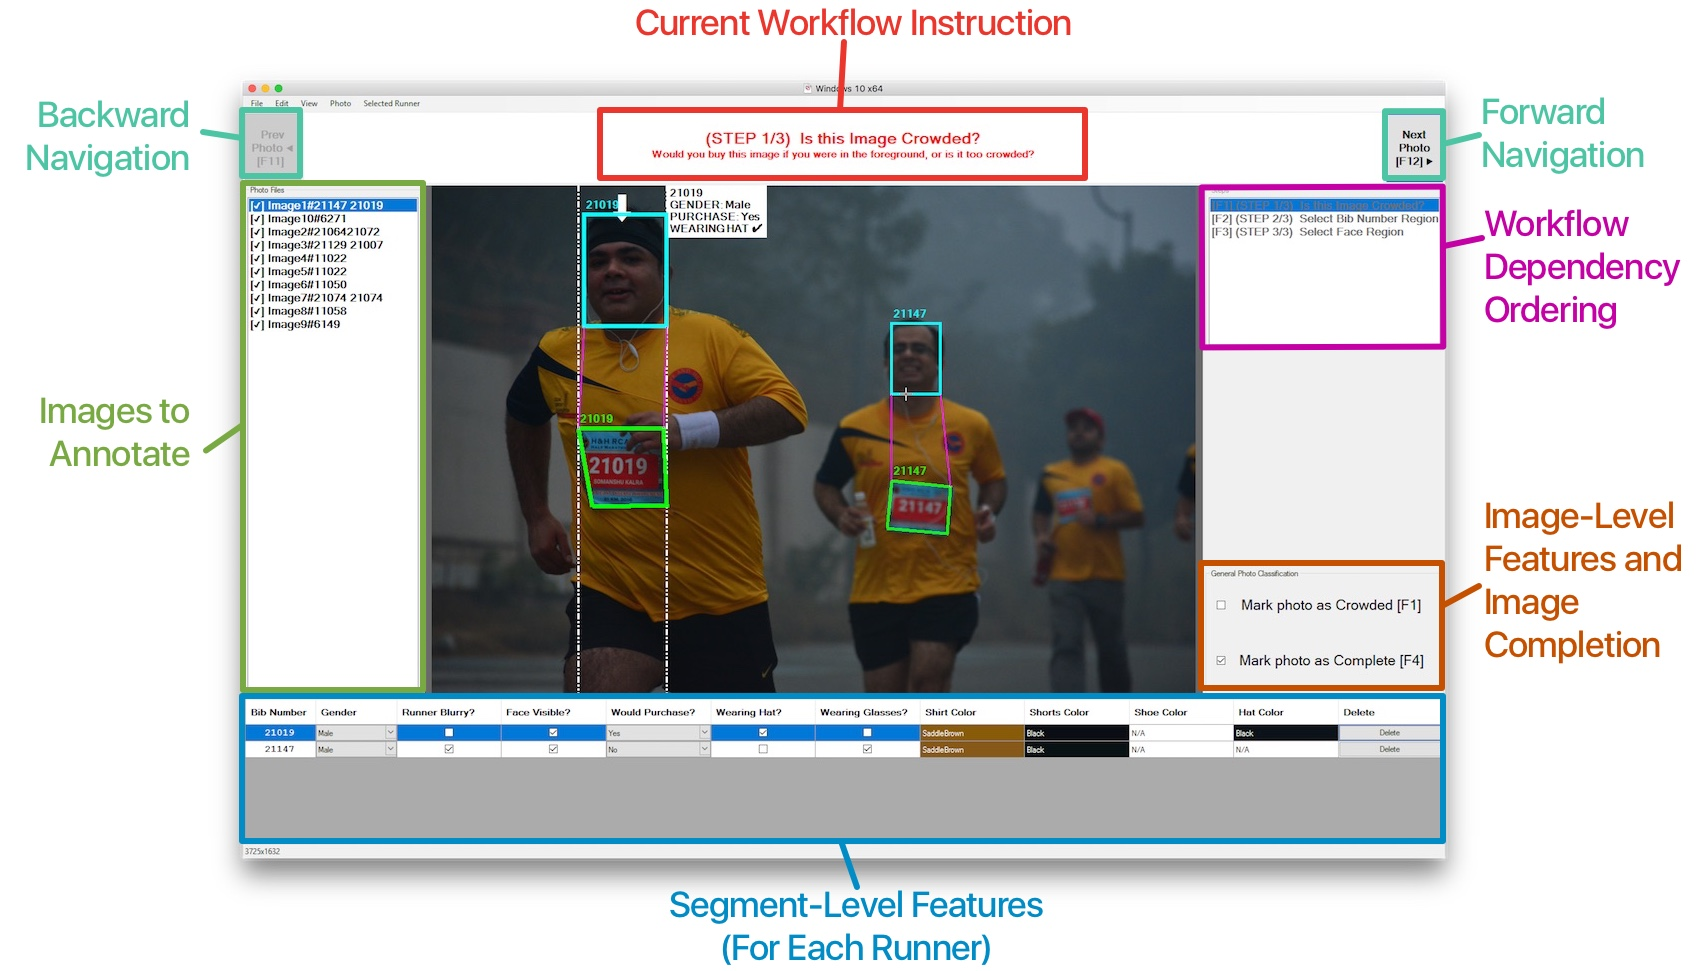
\includegraphics[width=\textwidth]{images/dataset/argus/argus_ui}
  \caption[An overview of the Argus user interface]{An overview of the Argus user interface.}
  \label{fig:dataset:argus:overview}
\end{figure}

\begin{figure}
  \centering
  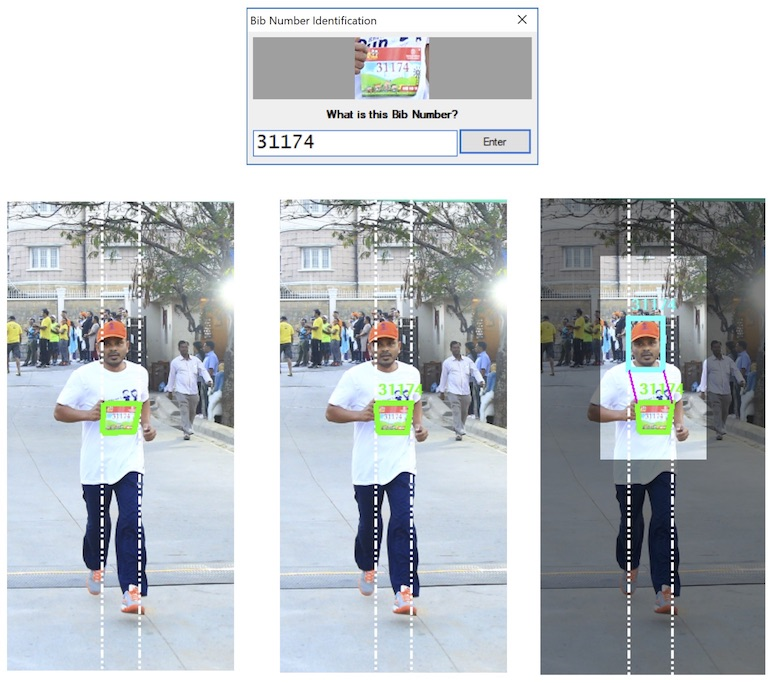
\includegraphics[width=\textwidth]{images/dataset/argus/argus_entry}
  \caption[Bib and Face feature annotation with Argus]{$Bib$ and $Face$ segment-level feature annotation. Users click four times around the bib to mark up the $BibSheet$ region (left). A dialog asks the user to enter the $\gls{rbn}$ label (top). The \gls{rbn} is annotated on the image (middle) and users can progress to drag-and-drop around the $Face$ region within the restrictions set (see \cref{sec:dataset:architecture:metamodel}). Note the dependency ordering is present.}
  \label{fig:dataset:argus:bib_and_face}
\end{figure}

\begin{figure}
  \hspace{\fill}
  \begin{subfigure}[b]{0.45\textwidth}
    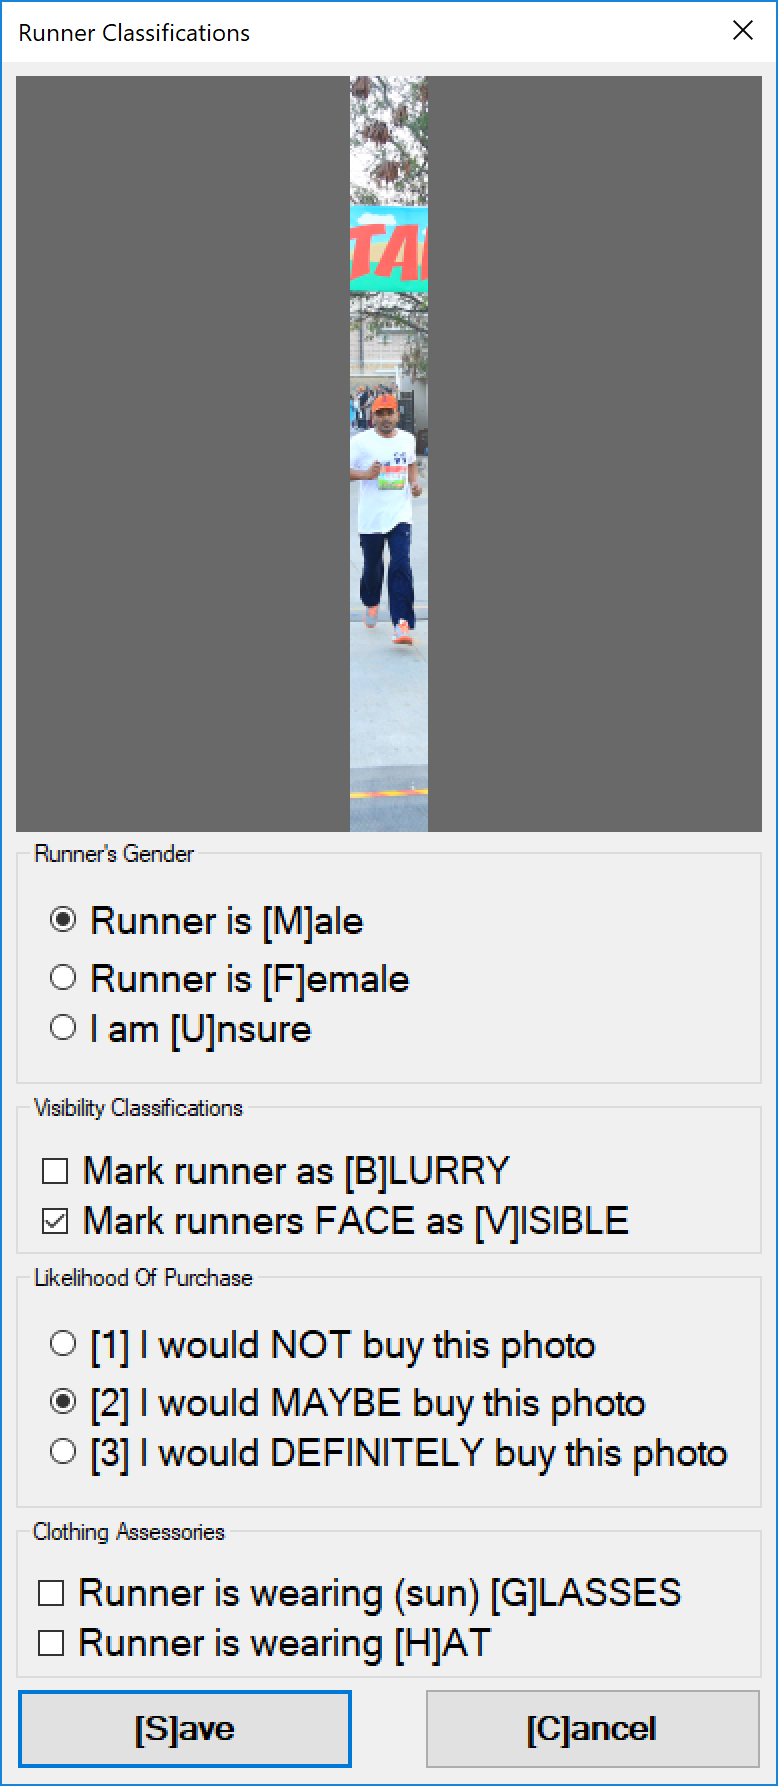
\includegraphics[width=\textwidth]{images/dataset/argus/argus_prom_entry}
  \end{subfigure}
  \hspace{\fill}
  \begin{subfigure}[b]{0.45\textwidth}
    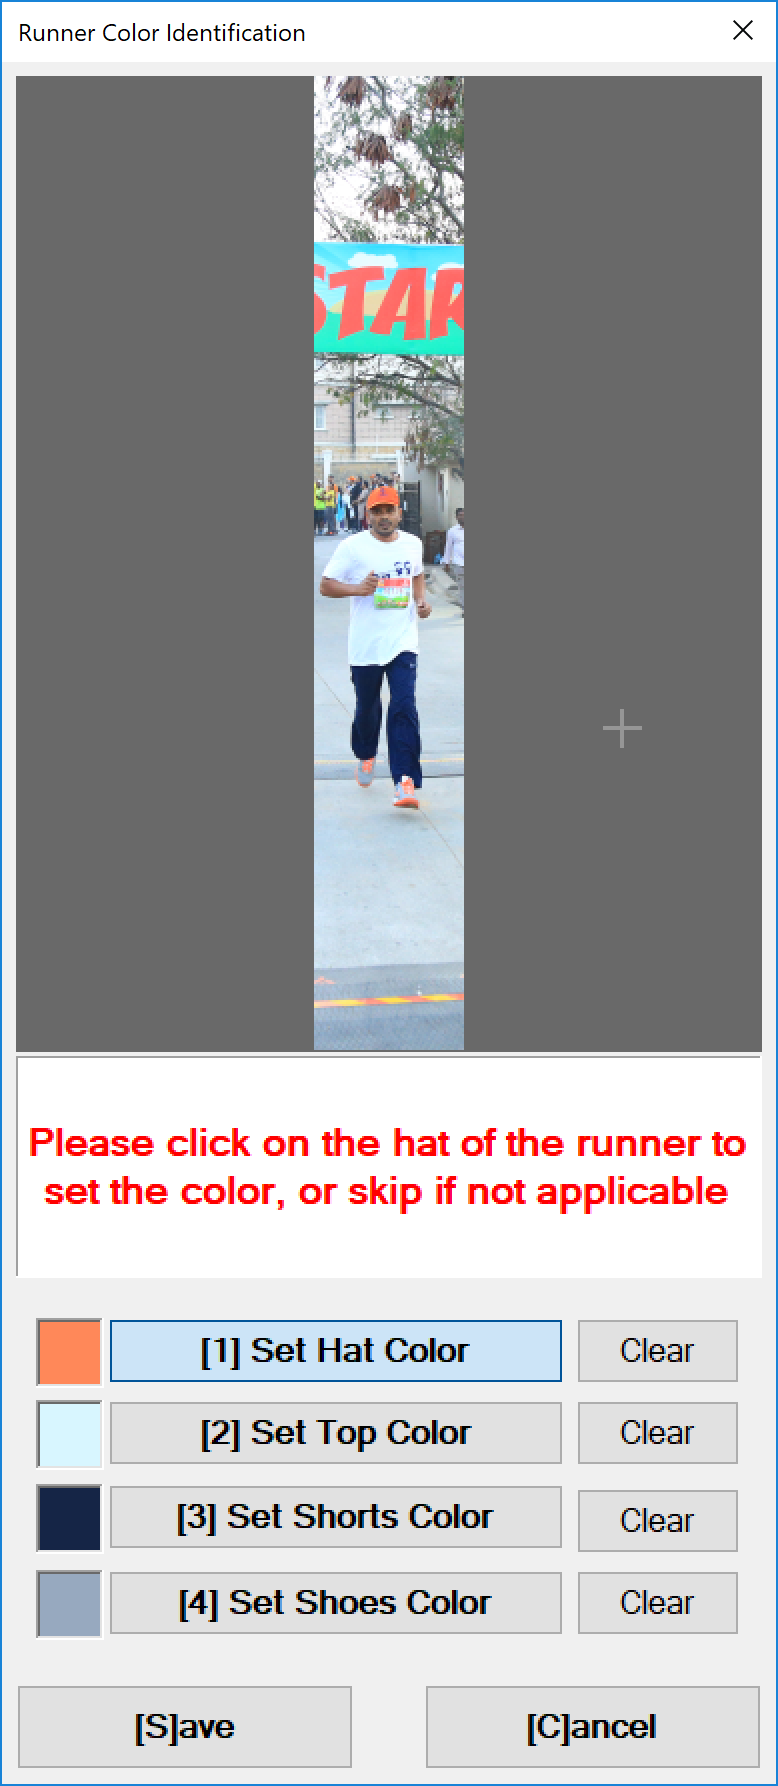
\includegraphics[width=\textwidth]{images/dataset/argus/argus_color_entry}
  \end{subfigure}
  \hspace{\fill}
  \caption[Prominence and Colour feature annotation with Argus]{Annotation for the $Prominence$ and $Colour$ segment-level features.}
  \label{fig:dataset:argus:prom_and_col}
\end{figure}

We deployed Argus to data taggers remotely using the ClickOnce Deployment\footnoteurl{https://msdn.microsoft.com/en-us/library/t71a733d.aspx}{11 August 2017} strategy.

\clearpage

\subsection{Annotation Throughput}
\label{sec:dataset:argus:metrics}

While Argus is running, we gathered a number of metrics to determine what throughput was achievable in our 803 images, presented in  \cref{fig:dataset:argus:metrics:throughput}. We measure throughput as either image-level of segment-level features. A single image usually takes less than a minute to markup, and the longest feature to markup is the prominence and face features, especially as we gather the most annotations here. These statistics may be useful for productivity analysis on how long a given dataset may take to markup using Argus, but we leave this area of investigation open for future works.

\begin{figure}[h]
  \begin{subfigure}[b]{\textwidth}
    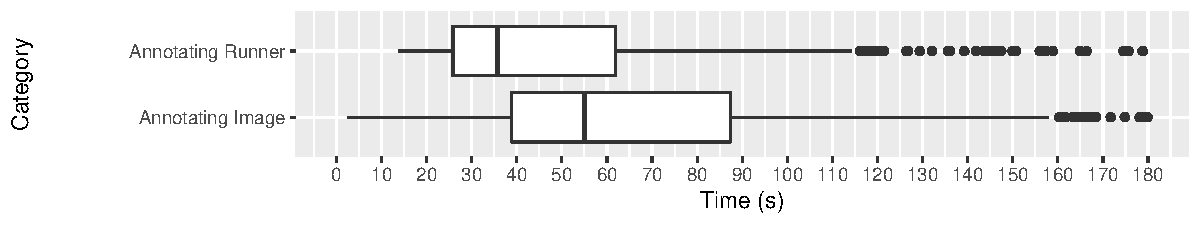
\includegraphics[width=\textwidth]{images/dataset/argus/photo_box_plots}
    \caption{Overall timing per image.}   
  \end{subfigure}
  \smallskip
  \\
  \begin{subfigure}[b]{\textwidth}
    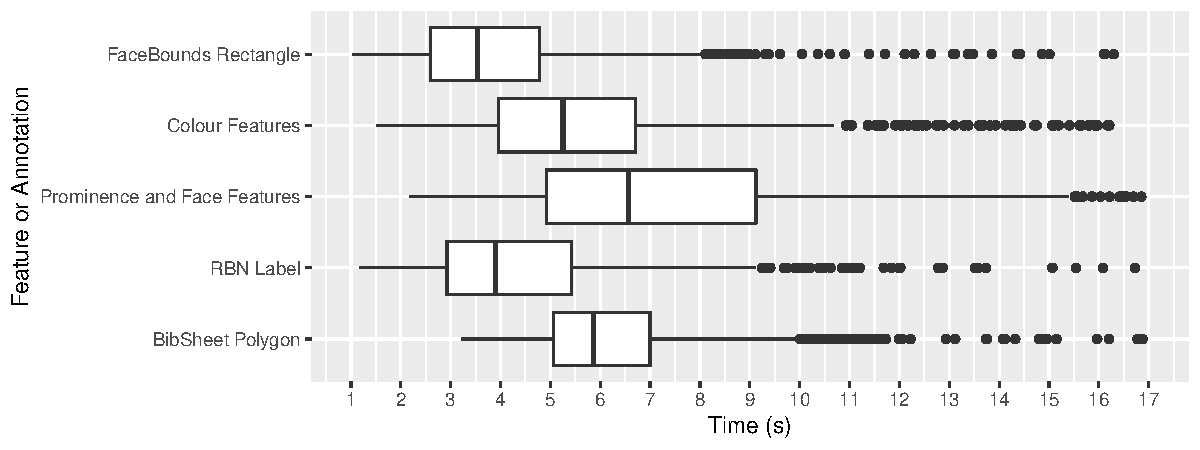
\includegraphics[width=\textwidth]{images/dataset/argus/feature_box_plots}
    \caption{Segment-level features and annotations marked up.}   
  \end{subfigure}
  \caption[Throughput of images using Argus]{Throughput of 803 images using Argus.}
  \label{fig:dataset:argus:metrics:throughput}
\end{figure}

Another metric gathered were the number of mistakes made during annotation. We define `mistake' as a rule violation, \gls{ui} violation, or poor data entry. As shown in \cref{tab:dataset:argus:metrics:mistakes}, it is quite clear how useful adding construction rules to our metamodel is---upon trials made using Argus, we needed to add the $FaceBounds$ restriction (\cref{fig:dataset:issues_with_tagging}), which was then violated a further 130 times during our annotation. \gls{ui} restrictions automatically built into Argus also proved useful. These restrictions  prevented users from dragging-and-dropping from bottom-right to top-left (inverse rectangle)\footnote{Although, it would have been possible to automatically swap the $x_{1}$ and $y_{1}$ with $x_{2}$ and $y_{2}$ within Argus.} or checking if a polygon was being dragged-and-dropped instead of clicked (and vice versa for rectangles).

\begin{table}[h]
  \centering
  \caption[Mistakes using Argus]{Frequencies of mistakes made during the annotation process. These are separated into construction rule violations, \gls{ui} violations, and poor data entry.}
  \label{tab:dataset:argus:metrics:mistakes}
  \begin{tabular}{@{}ll@{}}
    \toprule
    \textbf{Statistic}                                & \textbf{Frequency} \\ \midrule
    Marked as complete when $Face$ region not tagged  & 20                 \\
    Selected outside $FaceBounds$ restriction         & 130                \\
    Selected $FaceBounds$ below $BibSheet$            & 7                  \\
    \midrule
    Drag-and-drop inversely for $FaceBounds$          & 4                  \\
    Drag-and-drop made for $BibSheet$ polygon         & 73                 \\
    Clicked instead of drag-and-drop for $FaceBounds$ & 45                 \\
    \midrule
    Undos made                                        & 70                 \\
    Deleted runner annotation                         & 46                 \\ \bottomrule
  \end{tabular}
\end{table}

\subsection{Annotation \glsdisp{lop}{LoP} Bias}

Upon inspection of our \gls{lop} metrics, we found that, of all runner's that were annotated (1,031), 77.1\% were marked with a \gls{lop} of \textsc{yes}, 10.7\% were marked as \textsc{maybe} and 12.2\% were marked as \textsc{no}. These values are important for prominence ranking training, as we we know there are far more prominent runners (with a higher \gls{lop}) to train an \gls{ai} model. Furthermore, we want to reduce as many \textsc{maybe} \gls{lop} values as possible as these annotations are discarded in prominence training to reduce impartial bias when training a \gls{nn}---and as shown our dataset was annotated with the \textsc{maybe} values at a minimum. Augmentation (\cref{sec:dataset:postprocessing:augmentation}) is required to increase the number of \textsc{no} training samples.

\subsection{Annotation Quality Evaluation}
\label{sec:dataset:argus:quality_eval}

We took a subset of 260 randomly selected images  (approximately one third of the entire dataset) tagged from the data tagging team and assessed the photos for quality assurance. Here, we inspected photos on three tiers: `Good', `Okay' and `Bad' quality. We deemed photos as `Good' if there were no flaws at all with the tagging, `Okay' if there were minor errors made that we can compensate with, and `Bad' if there are significant flaws with the tagging that would affect the \gls{ai} model. Refer to \cref{fig:dataset:argus:qualituy_tiers} for samples of these images.

\begin{figure}
  \hspace{\fill}
  \begin{subfigure}[b]{0.30\textwidth}
    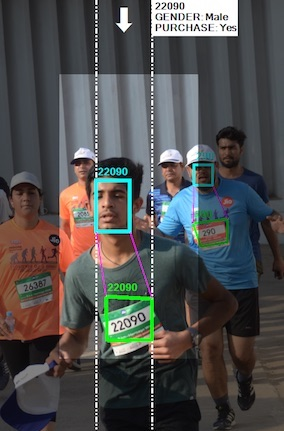
\includegraphics[width=\textwidth]{images/dataset/argus/quality_tagging_bad_polygons}
    \caption{A `Bad' annotation}
    \label{fig:dataset:argus:qualituy_tiers:bad_polygons}
  \end{subfigure}
  \hspace{\fill}
  \begin{subfigure}[b]{0.30\textwidth}
    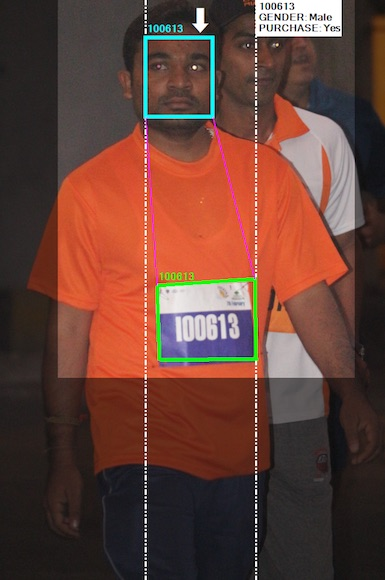
\includegraphics[width=\textwidth]{images/dataset/argus/quality_tagging_bad_invalid_rbn}
    \caption{A `Bad' annotation}
    \label{fig:dataset:argus:qualituy_tiers:bad_invalid_rbn}
  \end{subfigure}
  \hspace{\fill}
  \begin{subfigure}[b]{0.30\textwidth}
    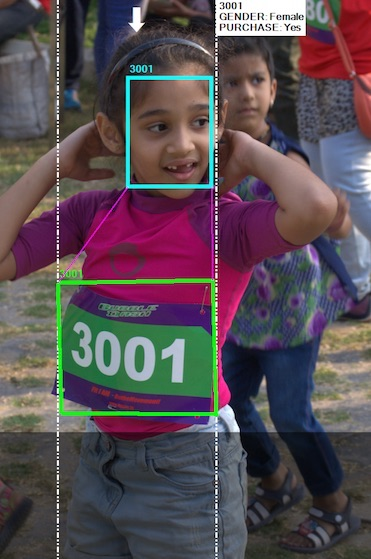
\includegraphics[width=\textwidth]{images/dataset/argus/quality_tagging_okay}
    \caption{An `Okay' annotation}
      \label{fig:dataset:argus:qualituy_tiers:okay}
  \end{subfigure}
  \hspace{\fill}
  \caption[Quality assurance using Argus]{`Okay' and `Bad' quality tagging tiers.}
  \label{fig:dataset:argus:qualituy_tiers}
\end{figure}

In \cref{fig:dataset:argus:qualituy_tiers:okay}, we see that the $FaceBounds$ annotation is too small around the runner's head, and that the $BibSheet$ polygon has been marked as a square, rather than directly around the four corners of the bib sheet. This is considered `Okay' as we are able to compensate with the extra padding around the $BibSheet$, and the $FaceBounds$ could have padding to extend the area. In \cref{fig:dataset:argus:qualituy_tiers:bad_polygons,fig:dataset:argus:qualituy_tiers:bad_invalid_rbn}, however, we are given completely incorrect information. In the former, the $BibSheet$ polygon is not at all reflective of the actual sheet, including part of the runner's shirt in the annotation, and the $FaceRegion$ is too small unless significant padding is added. In the latter, the $\gls{rbn}$ has been annotated with the value \texttt{\textbf{1}00613}, confusing the first character as numeric when it is alphabetic (\texttt{\textbf{I}00613}). As stipulated, these instances show significant fallbacks to quality that may hinder training the \gls{nn}.

In our sample set, we also evaluated whether the number of runner's in an overall photo has a negative impact on the annotation quality (\cref{fig:dataset:argus:quality_of_tagging_count}), as well as how long taggers spend on annotating photos (\cref{fig:dataset:argus:quality_of_tagging_count}). Upon analysis, we can see that most runners are actually well-annotated---only in images containing one runner where there are more `Bad' annotations than `Okay' ones, and generally `Okay' and `Good' outcomes are largely consistent regardless of runner count. Therefore, likelihood of time spent on annotations is `Good', and `Bad' marking distribution is more biased towards short evaluation times where there are few runners in the image. \cref{fig:dataset:argus:quality_of_tagging_count} confirms our hypothesis where, we can see, the longer the annotator spend time tagging, the better the quality of our data is: a mean of 48 seconds is improved to 52 seconds between `Bad' and `Okay', and this jumps to a mean of 55 seconds for `Good'. Therefore a difference in 7 seconds spend on tagging a photo, on average, shows a significant improvement on the quality of the tagging.

\begin{figure}[p]
  \centering
  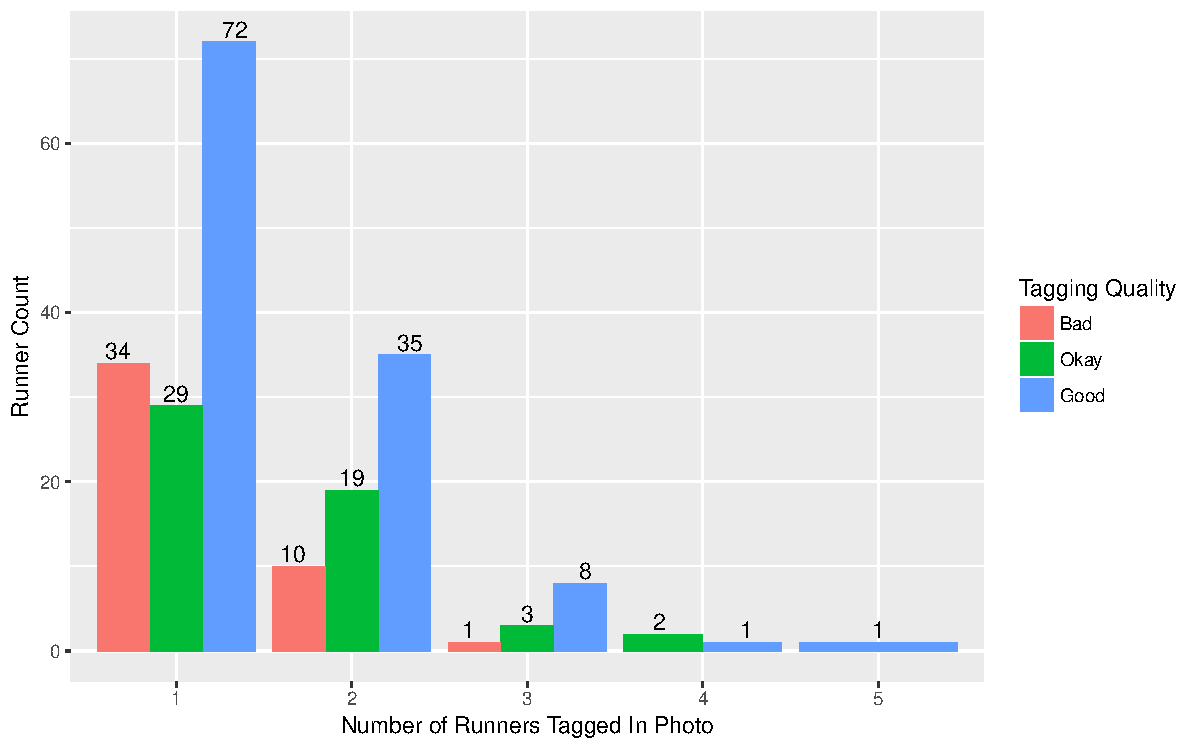
\includegraphics[width=0.9\textwidth]{images/dataset/argus/quality_of_tagging_count}
  \caption[Quality of tagging related the number of runners per photo]{The quality of tagging against the number of runners per photo.}
  \label{fig:dataset:argus:quality_of_tagging_count}
\end{figure}

\begin{figure}[p]
  \centering
  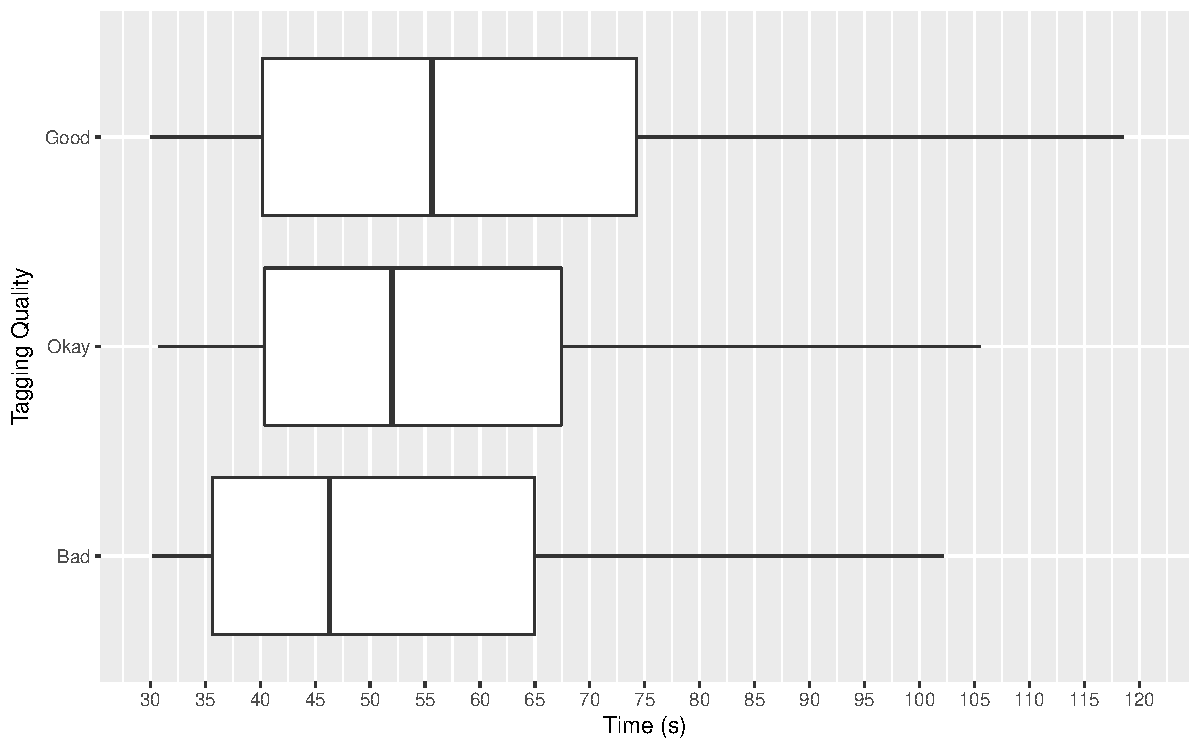
\includegraphics[width=0.9\textwidth]{images/dataset/argus/quality_of_tagging_time}
  \caption[Quality of tagging and seconds evaluating the photo]{Quality of tagging against the time spent evaluating the photo.}
  \label{fig:dataset:argus:quality_of_tagging_count}
\end{figure}

\clearpage